% Section 6.2, source PDF 78-90 / printed 68-80. Source-aligned staging, not yet accepted.
% block: exterior-calculus-section-heading page:78 type:section
\subsection{\BT{Exterior calculus}{外微积分}}\label{sec:exterior-calculus}

% block: exterior-calculus-fields pages:78,79 type:ordinary-paragraph
\BT{The primary objects of study in vector calculus are functions $\Omega\to\mathbb R$ and vector fields $\Omega\to\mathbb R^n$, defined on a domain $\Omega\subset\mathbb R^n$. In exterior calculus on $\mathbb R^n$, the primary objects are differential $k$-forms which are functions $\Omega\to\operatorname{Alt}^k\mathbb R^n$. In particular, the cases of functions and vector fields is included. Indeed, as we have seen, there are two different but natural ways to think of the functions of vector calculus as differential forms (either as $0$-forms or $n$-forms), and similarly vector fields may be identified with either $1$-forms or $(n-1)$-forms. This distinction, which is lost in vector calculus, turns out to be a strength of exterior calculus. Maxwell referred to it when he wrote that "physical vector quantities may be divided into two classes, in one of which the quantity is defined with reference to a line, while in the other the quantity is defined with reference to an area" \BookCite{58}. In higher dimensions other types of fields arise. For example, a differential $2$-form in four dimensions is a field with six independent components (the number of independent components in a $4\times4$ skew-symmetric matrix).}{向量微积分的主要研究对象是在区域 $\Omega\subset\mathbb R^n$ 上定义的函数 $\Omega\to\mathbb R$ 和向量场 $\Omega\to\mathbb R^n$. 在 $\mathbb R^n$ 上的外微积分中, 主要对象是微分 $k$-形式, 即函数 $\Omega\to\operatorname{Alt}^k\mathbb R^n$. 特别地, 它包含函数和向量场的情形. 事实上, 如前所见, 可以用两种不同而自然的方式将向量微积分中的函数看作微分形式 (或者是 $0$-形式, 或者是 $n$-形式), 类似地, 向量场可以与 $1$-形式或 $(n-1)$-形式等同. 这种在向量微积分中丢失的区别, 恰恰成为外微积分的优点. Maxwell 写道, "物理向量量可以分为两类, 一类参照线来定义, 另一类则参照面积来定义" \BookCite{58}, 说的就是这一点. 在更高维中还会出现其他类型的场. 例如, 四维中的微分 $2$-形式是具有六个独立分量的场 (即 $4\times4$ 反对称矩阵中独立分量的个数).}

% block: exterior-calculus-manifold-generality page:79 type:ordinary-paragraph
\BT{Actually exterior calculus develops most naturally if we are more general, permitting as the domain $\Omega$ any manifold (finite dimensional, with or without boundary, and smooth enough that tangent spaces are defined), not just open subsets in $\mathbb R^n$. Much of the theory works in this degree of generality, depending only on the differentiable structure of the domain. Other concepts require additional structure: either an inner product (i.e., a Riemannian manifold), or an orientation (an oriented manifold), or both, and some formulas simplify if we use a preferred basis. Of course, a domain on $\mathbb R^n$ is endowed with all these things. But it is enlightening to hold clearly in mind what structures are required for what operations, as we shall do. From a practical point of view, even if we are only interested in solving boundary value problems in $\mathbb R^n$, we will need differential forms not only on the domain where the differential equation is defined but also on its boundary---which is a manifold, but not a domain in Euclidean space.}{实际上, 若采取更一般的观点, 允许区域 $\Omega$ 为任意流形 (有限维, 有边界或无边界, 并且足够光滑以使切空间有定义), 而不只是 $\mathbb R^n$ 中的开子集, 外微积分的展开就最为自然. 理论的很大一部分在这种一般程度下都成立, 只依赖区域的可微结构. 其他概念则需要附加结构: 内积 (即 Riemannian 流形), 或定向 (有定向流形), 或两者兼具; 使用特选基还可以简化某些公式. 当然, $\mathbb R^n$ 中的区域具有所有这些结构. 但像我们将要做的那样, 清楚记住何种运算需要何种结构, 很有启发性. 从实用角度看, 即使只关心求解 $\mathbb R^n$ 中的边值问题, 也不仅需要在定义微分方程的区域上使用微分形式, 还需要在其边界上使用; 边界是流形, 但不是 Euclidean 空间中的区域.}

% block: differential-forms-heading page:79 type:subsection
\subsubsection{\BT{Differential forms}{微分形式}}\label{subsec:differential-forms}

% block: tangent-bundle-sections page:79 type:ordinary-paragraph
\BT{Let $\Omega$ be a manifold of dimension $n$. At each point $x\in\Omega$, the tangent space $T_x\Omega$ is a vector space of dimension $n$, and the collection of all pairs $(x,v)$ with $x\in\Omega$ and $v\in T_x\Omega$ defines the tangent bundle, which is a manifold of dimension $2n$. A \emph{section} of this bundle is a function from $\Omega$ to its tangent bundle which assigns to each $x\in\Omega$ a tangent vector $v_x\in T_x\Omega$. That is, it is a tangent vector field.}{设 $\Omega$ 是维数为 $n$ 的流形. 在每个点 $x\in\Omega$ 处, 切空间 $T_x\Omega$ 是维数为 $n$ 的向量空间; 所有满足 $x\in\Omega$ 和 $v\in T_x\Omega$ 的二元组 $(x,v)$ 的集合定义了切丛, 它是维数为 $2n$ 的流形. 此丛的一个\emph{截面}是从 $\Omega$ 到其切丛的函数, 为每个 $x\in\Omega$ 指定一个切向量 $v_x\in T_x\Omega$. 也就是说, 它是切向量场.}

% block: differential-form-bundle page:79 type:ordinary-paragraph
\BT{Applying the exterior algebra constructions of the previous section, we may define a bundle (the $k$th exterior power of the cotangent bundle) consisting of pairs $(x,\mu)$ with $\mu\in\operatorname{Alt}^kT_x\Omega$. A \emph{differential $k$-form} is a section of this bundle, i.e., a function which assigns to each $x\in\Omega$ an element of $\operatorname{Alt}^kT_x\Omega$. Thus $\omega$ being a differential $k$-form means that}{应用上一节的外代数构造, 可以定义一个丛 (余切丛的第 $k$ 次外幂), 由满足 $\mu\in\operatorname{Alt}^kT_x\Omega$ 的二元组 $(x,\mu)$ 构成. \emph{微分 $k$-形式}就是此丛的一个截面, 即为每个 $x\in\Omega$ 指定 $\operatorname{Alt}^kT_x\Omega$ 中一个元素的函数. 因此, $\omega$ 为微分 $k$-形式意味着}
\[
\omega_x(v_1,\ldots,v_k)\in\mathbb R\quad\forall x\in\Omega,\ v_1,\ldots,v_k\in T_x\Omega,
\]
\BT{with the dependence on the vectors $v_i$ being multilinear and alternating. We will usually require some degree of smoothness for the dependence on $x$, varying with the context. In the case where $\Omega$ is indeed a subdomain of $\mathbb R^n$, we may identify all the tangent spaces with $\mathbb R^n$, and so a differential $k$-form is just a function $\Omega\to\operatorname{Alt}^k\mathbb R^n$. It may be written as}{其中对向量 $v_i$ 的依赖是多重线性且交错的. 通常还要求对 $x$ 的依赖具有某种光滑性, 具体程度随上下文而定. 当 $\Omega$ 确为 $\mathbb R^n$ 的子区域时, 可将所有切空间与 $\mathbb R^n$ 等同, 因而微分 $k$-形式就是函数 $\Omega\to\operatorname{Alt}^k\mathbb R^n$. 它可写为}
\begin{equation}\label{eq:differential-form-coordinates}
\omega=\sum_{1\leq\sigma_1<\cdots<\sigma_k\leq n}a_\sigma\,dx^{\sigma_1}\wedge\cdots\wedge dx^{\sigma_k},
\end{equation}
\BT{with the coefficients $a_\sigma$ real-valued functions on $\Omega$.}{其中系数 $a_\sigma$ 是 $\Omega$ 上的实值函数.}

% block: differential-form-space-notation page:79 type:ordinary-paragraph
\BT{We write $\Lambda^k(\Omega)$, or just $\Lambda^k$, for the vector space of differential $k$-forms on $\Omega$ when we do not need to emphasize the exact degree of smoothness expected. When we do, we will precede the notation with a function space. For example, $C\Lambda^k$ denotes the space of continuous differential forms, $C^1\Lambda^k$ of continuously differentiable forms, etc. We will introduce notation for spaces with different specified levels of smoothness below.}{不需要强调所要求的精确光滑程度时, 将 $\Omega$ 上的微分 $k$-形式向量空间记为 $\Lambda^k(\Omega)$, 或简称 $\Lambda^k$. 需要强调时, 则在这一记号之前加上函数空间. 例如, $C\Lambda^k$ 表示连续微分形式空间, $C^1\Lambda^k$ 表示连续可微形式空间, 等等. 下面将引入具有不同指定光滑程度的空间的记号.}

% block: differential-form-pointwise-operations page:80 type:ordinary-paragraph
\medskip\noindent\textbf{\BT{Exterior product, contraction, inner product, Hodge star, vector proxies}{外积, 缩并, 内积, Hodge 星算子, 向量代理}}\par
\BT{The algebraic operations on alternating multilinear forms discussed in the previous section can be applied to differential forms pointwise. For example, the exterior product of $\omega\in\Lambda^j$ and $\mu\in\Lambda^k$ is a differential $(j+k)$-form given by}{上一节讨论的交错多重线性形式上的代数运算, 可以逐点应用于微分形式. 例如, $\omega\in\Lambda^j$ 和 $\mu\in\Lambda^k$ 的外积是如下微分 $(j+k)$-形式:}
\[
(\omega\wedge\mu)_x=\omega_x\wedge\mu_x.
\]
\BT{Similarly, if $v$ is a vector field on $\Omega$ and $\omega\in\Lambda^k(\Omega)$, then $\omega\lrcorner v$ is a differential $(k-1)$-form. In order to extend the operations that need an inner product, we require the manifold $\Omega$ to be Riemannian, so that at each point $x$ there is given an inner product on $T_x\Omega$. The inner product should depend smoothly on $x$ in the sense that if $v_x$ and $w_x$ are smooth vector fields, then $x\mapsto\langle v_x,w_x\rangle_{T_x\Omega}$ should be a smooth function on $\Omega$ (the exact degree of smoothness again depending on the context). Several of the algebraic operations also require an orientation of the tangent spaces $T_x\Omega$ and we suppose that these have been assigned at each point in a consistent fashion. This requires that the manifold be orientable. It is not possible, for example, on a Möbius strip. On an oriented Riemannian manifold, there is a unique volume $n$-form, characterized by the fact that at each point $x$ it assigns the value $1$ to each positively oriented orthonormal basis of $T_x\Omega$. The Hodge star operator from $\Lambda^k$ to $\Lambda^{n-k}$ is then defined pointwise by \eqref{eq:hodge-star-characterization}, and we can compute the inner product in $L^2\Lambda^k(\Omega)$ by}{类似地, 若 $v$ 是 $\Omega$ 上的向量场且 $\omega\in\Lambda^k(\Omega)$, 则 $\omega\lrcorner v$ 是微分 $(k-1)$-形式. 为延拓需要内积的运算, 要求流形 $\Omega$ 是 Riemannian 流形, 即在每点 $x$ 处的 $T_x\Omega$ 上给定内积. 内积应光滑地依赖于 $x$, 即若 $v_x$ 和 $w_x$ 是光滑向量场, 则 $x\mapsto\langle v_x,w_x\rangle_{T_x\Omega}$ 应为 $\Omega$ 上的光滑函数 (确切的光滑程度仍由上下文决定). 一些代数运算还需要切空间 $T_x\Omega$ 的定向, 并假设在各点以一致方式指定了这些定向. 这要求流形可定向. 例如在 Möbius 带上就不可能做到. 在有定向 Riemannian 流形上, 存在唯一的体积 $n$-形式, 其特征是在每点 $x$ 处, 将 $T_x\Omega$ 的每组正向标准正交基映为值 $1$. 随后由 \eqref{eq:hodge-star-characterization} 逐点定义从 $\Lambda^k$ 到 $\Lambda^{n-k}$ 的 Hodge 星算子, 并可按下式计算 $L^2\Lambda^k(\Omega)$ 中的内积:}
\[
\langle\omega,\nu\rangle_{L^2\Lambda^k}=\int_\Omega\langle\omega,\nu\rangle\operatorname{vol}=\int_\Omega\omega\wedge\star\nu,\qquad\omega,\nu\in L^2\Lambda^k(\Omega).
\]
\BT{Applying the vector proxies pointwise, we can identify differential $0$-forms and differential $n$-forms with real-valued functions on the manifold and identify differential $1$-forms and differential $(n-1)$-forms with tangential vector fields.}{逐点应用向量代理, 可将微分 $0$-形式和微分 $n$-形式与流形上的实值函数等同, 将微分 $1$-形式和微分 $(n-1)$-形式与切向量场等同.}

% block: smooth-pullback page:80 type:ordinary-paragraph
\begingroup\emergencystretch=1em
\medskip\noindent\textbf{\BT{Pullback under smooth maps and traces}{光滑映射下的拉回与迹}}\par
\BT{If $\phi:M\to N$ is a differentiable map between manifolds, its derivative $\phi'(x)$ is a linear map of $T_xM$ to $T_{\phi(x)}N$. If $\omega\in\Lambda^k(N)$, we may therefore define a differential $k$-form on $\Omega$ by}{若 $\phi:M\to N$ 是流形之间的可微映射, 则其导数 $\phi'(x)$ 是从 $T_xM$ 到 $T_{\phi(x)}N$ 的线性映射. 若 $\omega\in\Lambda^k(N)$, 则可由下式定义 $\Omega$ 上的微分 $k$-形式:}
\begin{equation}\label{eq:smooth-pullback-definition}
(\phi^*\omega)_x=\phi'(x)^*\omega_{\phi(x)},
\end{equation}
\BT{where, on the right-hand side, we are using the algebraic pullback defined by \eqref{eq:linear-pullback-definition}. This defines the pullback $\phi^*\omega\in\Lambda^k(M)$ of a differential form under a smooth map. As in the algebraic case, pullback acts contravariantly and respects the exterior product.}{其中右端使用了 \eqref{eq:linear-pullback-definition} 定义的代数拉回. 这就定义了光滑映射下微分形式的拉回 $\phi^*\omega\in\Lambda^k(M)$. 与代数情形一样, 拉回反变地作用并保持外积.}

\par\endgroup
% block: differential-trace-proxies pages:80,81 type:ordinary-paragraph
\BT{The pullback of the inclusion of a submanifold $M$ into another manifold $N$ is called the trace operator, denoted $\operatorname{tr}:\Lambda^k(N)\to\Lambda^k(M)$. In the case of $0$-forms it is just restriction of functions. The derivative of the inclusion at a point $x\in M$ is the inclusion of $T_xM\subset T_xN$. This fact and our calculations at the end of Section~\ref{subsec:alternating-form-operations} provide formulas for the trace in terms of proxies in two important cases. If $w$ is a vector field on $N$ corresponding to some $1$-form $\omega\in\Lambda^1(N)$, then the vector field $\bar w$ on $M$ corresponding to $\operatorname{tr}\omega\in\Lambda^1(M)$ is given by}{子流形 $M$ 到另一流形 $N$ 的包含映射的拉回称为迹算子, 记为 $\operatorname{tr}:\Lambda^k(N)\to\Lambda^k(M)$. 对 $0$-形式, 它就是函数的限制. 包含映射在点 $x\in M$ 处的导数, 就是 $T_xM\subset T_xN$ 的包含映射. 这一事实结合 Section~\ref{subsec:alternating-form-operations} 末尾的计算, 给出了两种重要情形下用代理表示的迹公式. 若 $w$ 是 $N$ 上对应于某个 $1$-形式 $\omega\in\Lambda^1(N)$ 的向量场, 则 $M$ 上对应于 $\operatorname{tr}\omega\in\Lambda^1(M)$ 的向量场 $\bar w$ 由下式给出:}
\[
\bar w(x)=\pi w(x),\qquad x\in M,
\]
\BT{where $\pi=\pi_{T_xM}:T_xN\to T_xM$ is the orthogonal projection. If instead $\dim M=\dim N-1$ and the vector field $w$ corresponds to $\omega\in\Lambda^{\dim N-1}(N)$, then $\operatorname{tr}\omega$ corresponds to the scalar function $\langle w,n\rangle$ on $M$, where $n$ is the appropriately oriented unit normal to $M$ in $N$.}{其中 $\pi=\pi_{T_xM}:T_xN\to T_xM$ 是正交投影. 如果 $\dim M=\dim N-1$, 且向量场 $w$ 对应于 $\omega\in\Lambda^{\dim N-1}(N)$, 则 $\operatorname{tr}\omega$ 对应于 $M$ 上的标量函数 $\langle w,n\rangle$, 其中 $n$ 是 $M$ 在 $N$ 中适当定向的单位法向量.}

% block: coordinate-trace page:81 type:ordinary-paragraph
\BT{In the case $M=\mathbb R^{n-1}$, $N=\mathbb R^n$, with the inclusion given by $x\mapsto(0,x)$, we can write the corresponding trace operator in terms of coordinates. If $\omega$ is the differential form given by \eqref{eq:differential-form-coordinates}, then}{当 $M=\mathbb R^{n-1}$, $N=\mathbb R^n$, 且包含映射为 $x\mapsto(0,x)$ 时, 可用坐标写出相应的迹算子. 若 $\omega$ 是 \eqref{eq:differential-form-coordinates} 给出的微分形式, 则}
\begin{equation}\label{eq:differential-trace-coordinates}
\operatorname{tr}\omega=\sum_{\{\sigma\mid\sigma_1>1\}}(\operatorname{tr}a_\sigma)\,dx^{\sigma_1}\wedge\cdots\wedge dx^{\sigma_k}.
\end{equation}
\BT{The trace operator appearing in the term $\operatorname{tr}a_\sigma$ on the right-hand side is the $0$-form trace, which is just the restriction to $\mathbb R^{n-1}$.}{右端 $\operatorname{tr}a_\sigma$ 中的迹算子是 $0$-形式的迹, 即在 $\mathbb R^{n-1}$ 上的限制.}

% block: exterior-derivative-heading page:81 type:subsection
\subsubsection{\BT{Exterior derivative}{外微分}}\label{subsec:exterior-derivative}

% block: exterior-derivative-definition page:81 type:ordinary-paragraph
\BT{The exterior derivative, which maps $\Lambda^k(\Omega)$ to $\Lambda^{k+1}(\Omega)$, is the fundamental operator of exterior calculus. It is simplest to define when $\Omega$ is a domain in $\mathbb R^n$. If $\omega$ is a smooth differential $k$-form, and $v_1,\ldots,v_k$ are $k$ vectors in $\mathbb R^n$, then $\omega_x(v_1,\ldots,v_k)$ is a differentiable function of $x$, which is alternating multilinear in the $k$ vectors. If $v_0$ is an additional vector, then we may apply $\partial_{v_0}:=v_0\cdot\operatorname{grad}$, the directional derivative in the direction $v_0$, to this function, obtaining a quantity which depends on $x$ and all $(k+1)$-vectors. The dependence on the vectors is linear in each but is not alternating. To get a $(k+1)$-form we take the alternating part. Multiplying this by $k+1$ gives the exterior derivative $d\omega$:}{将 $\Lambda^k(\Omega)$ 映到 $\Lambda^{k+1}(\Omega)$ 的外微分, 是外微积分的基本算子. 当 $\Omega$ 是 $\mathbb R^n$ 中的区域时, 定义最为简单. 若 $\omega$ 是光滑微分 $k$-形式, $v_1,\ldots,v_k$ 是 $\mathbb R^n$ 中的 $k$ 个向量, 则 $\omega_x(v_1,\ldots,v_k)$ 是 $x$ 的可微函数, 并且关于这 $k$ 个向量是交错多重线性的. 若再给定向量 $v_0$, 则可将沿 $v_0$ 方向的方向导数 $\partial_{v_0}:=v_0\cdot\operatorname{grad}$ 应用于此函数, 得到依赖于 $x$ 和全部 $(k+1)$ 个向量的量. 它对每个向量的依赖是线性的, 但并不交错. 为得到 $(k+1)$-形式, 取其交错部分. 再乘以 $k+1$, 就得到外微分 $d\omega$:}
\[
(d\omega)_x(v_0,\ldots,v_k)=\sum_{j=0}^k(-)^j\partial_{v_j}\omega_x(v_0,\ldots,\widehat{v_j},\ldots,v_k).
\]

% block: exterior-derivative-coordinates page:81 type:ordinary-paragraph
\BT{Written in terms of the standard coordinates on $\mathbb R^n$, a general element of $\Lambda^k(\Omega)$ can be written as}{用 $\mathbb R^n$ 上的标准坐标, $\Lambda^k(\Omega)$ 的一般元素可写为}
\[
\omega=\sum_{1\leq\sigma_1<\cdots<\sigma_k\leq n}f_\sigma\,dx^{\sigma_1}\wedge\cdots\wedge dx^{\sigma_k},
\]
\BT{where the coefficients $f_\sigma$ are functions on $\Omega$. Then}{其中系数 $f_\sigma$ 是 $\Omega$ 上的函数. 则}
\begin{equation}\label{eq:exterior-derivative-coordinates}
d\omega=\sum_\sigma\sum_{j=1}^n\frac{\partial f_\sigma}{\partial x^j}\,dx^j\wedge dx^{\sigma_1}\wedge\cdots\wedge dx^{\sigma_k}.
\end{equation}

% block: exterior-derivative-vector-calculus page:81 type:ordinary-paragraph
\BT{In the case $k=0$, for example, we have the formula}{例如当 $k=0$ 时, 有公式}
\[
df=\sum_{j=1}^n\frac{\partial f}{\partial x^j}\,dx^j.
\]
\BT{Identifying the $1$-form on the right-hand side with a vector field, we see that the exterior derivative on a $1$-form on $\mathbb R^n$ is just the gradient operator. Similar considerations show that the exterior derivative on an $(n-1)$-form can be identified with the divergence operator. In three dimensions, the exterior derivative on $1$-forms can be viewed as a mapping from vector fields to vector fields and is found to be the curl operator. Thus, in this case the entire de Rham complex \eqref{eq:differential-forms-de-rham-complex} can be expressed in the terminology of vector calculus as in \eqref{eq:vector-calculus-de-rham-complex}.}{将右端的 $1$-形式与向量场等同, 可见 $\mathbb R^n$ 上作用于 $1$-形式的外微分就是梯度算子. 类似的考虑表明, 作用于 $(n-1)$-形式的外微分可以与散度算子等同. 在三维中, 作用于 $1$-形式的外微分可视为从向量场到向量场的映射, 并可知它就是旋度算子. 因此, 此时整个 de Rham 复形 \eqref{eq:differential-forms-de-rham-complex} 都可用向量微积分的术语写成 \eqref{eq:vector-calculus-de-rham-complex}.}

% block: exterior-derivative-pullback-invariance page:82 type:ordinary-paragraph
\BT{An important property of the exterior derivative is that it is invariant under pullback. If $\phi:\Omega\to M$ is a map from a subdomain of $\mathbb R^n$ to a subdomain of $\mathbb R^m$, and $\omega\in\Lambda^k(M)$, then $\phi^*\omega\in\Lambda^k(\Omega)$ and}{外微分的一个重要性质是, 它在拉回下不变. 若 $\phi:\Omega\to M$ 是从 $\mathbb R^n$ 的子区域到 $\mathbb R^m$ 的子区域的映射, 且 $\omega\in\Lambda^k(M)$, 则 $\phi^*\omega\in\Lambda^k(\Omega)$, 并有}
\begin{equation}\label{eq:exterior-derivative-pullback}
d\phi^*\omega=\phi^*d\omega.
\end{equation}
\BT{In the case where $\phi$ is a diffeomorphism between two domains of equal dimension, we conclude that}{若 $\phi$ 是两个同维区域之间的微分同胚, 则得到}
\begin{equation}\label{eq:exterior-derivative-chart-definition}
d\omega=(\phi^{-1})^*d\phi^*\omega.
\end{equation}
\BT{We may use this formula to define $d\omega$ when $M$ is a manifold rather than a domain in Euclidean space. We choose any chart $\phi$ mapping some $\Omega\subset\mathbb R^n$ onto an open set of $M$ and then use the formula \eqref{eq:exterior-derivative-chart-definition} to define $d\omega$ on that open subset. Since $M$ is covered by charts, in this way we define $d\omega\in\Lambda^k(M)$. That the definition does not depend on the choice of charts follows from \eqref{eq:exterior-derivative-pullback}. Moreover this invariance under pullback holds for any smooth maps between manifolds.}{当 $M$ 是流形而不是 Euclidean 空间中的区域时, 可用此公式定义 $d\omega$. 任选将某个 $\Omega\subset\mathbb R^n$ 映到 $M$ 的一个开集上的坐标图 $\phi$, 再用公式 \eqref{eq:exterior-derivative-chart-definition} 定义该开子集上的 $d\omega$. 由于 $M$ 被坐标图覆盖, 由此就定义了 $d\omega\in\Lambda^k(M)$. 由 \eqref{eq:exterior-derivative-pullback} 可知, 此定义不依赖坐标图的选取. 此外, 这种拉回不变性对流形之间的任意光滑映射都成立.}

% block: exterior-differential-leibniz page:82 type:ordinary-paragraph
\BT{Another essential property of the exterior derivative is that it is a differential in the sense that $d\circ d=0$. It is enough to verify this on a domain in $\mathbb R^n$, where it follows easily from \eqref{eq:exterior-derivative-coordinates} thanks to the commutativity of partial derivatives. Equally essential is the Leibniz rule}{外微分的另一个基本性质是, 它是满足 $d\circ d=0$ 意义下的微分. 只需在 $\mathbb R^n$ 中的区域上验证这一点, 在那里由偏导数的交换性, 很容易从 \eqref{eq:exterior-derivative-coordinates} 得出结论. 同样重要的是 Leibniz 法则}
\begin{equation}\label{eq:exterior-leibniz-rule}
d(\omega\wedge\mu)=d\omega\wedge\mu+(-)^k\omega\wedge d\mu,\qquad\omega\in\Lambda^k(\Omega),\ \mu\in\Lambda^j(\Omega).
\end{equation}
\BT{It is worth emphasizing that the exterior derivative is defined without any reference to an inner product (metric) or an orientation on the manifold. A differential $k$-form on any manifold can be differentiated to give a differential $(k+1)$-form.}{值得强调的是, 外微分的定义完全不涉及流形上的内积 (度量) 或定向. 任意流形上的微分 $k$-形式都可以微分, 得到微分 $(k+1)$-形式.}

% block: differential-form-integration-heading page:82 type:subsection
\subsubsection{\BT{Integration of differential forms}{微分形式的积分}}\label{subsec:differential-form-integration}

% block: integration-orientation page:82 type:ordinary-paragraph
\BT{A differential $k$-form can be integrated over an oriented $k$-dimensional manifold to give a real number. Notice that the form degree and the manifold dimension must be the same. No metric or measure is required on the manifold to define the integral, and if they exist, then the integral is independent of them. However, the orientation does matter. If we switch it, the sign of the integral changes.}{微分 $k$-形式可以在有定向的 $k$ 维流形上积分, 得到实数. 注意, 形式次数必须与流形维数相同. 定义积分不需要流形上的度量或测度, 即使存在这些结构, 积分也与它们无关. 但定向确实重要. 改变定向就会改变积分的符号.}

% block: integration-parallelepiped-definition page:82 type:ordinary-paragraph
\BT{To get a basic idea of how the integral is defined, consider a parallelepiped $P$ determined by a point $x\in\mathbb R^k$ and $k$ linearly independent vectors $v_1,\ldots,v_k$, as in Figure~\ref{fig:integration-parallelograms}(a). If $\omega$ is a constant $k$-form on $P$, then the integral of $\omega$ over $P$ is simply $\omega_x(v_1,\ldots,v_k)$. If $\omega$ is smooth, but not constant, then this will be a good approximation of the integral if the parallelepiped is sufficiently small. Now any manifold can be approximated arbitrarily well by a collection of small tangent parallelopideds using coordinate charts, as illustrated in Figure~\ref{fig:integration-parallelograms}(b). We then get an approximate value for the integral by evaluating $\omega$ on each parallelogram and adding}{为初步理解积分如何定义, 考虑由一点 $x\in\mathbb R^k$ 和 $k$ 个线性无关向量 $v_1,\ldots,v_k$ 确定的平行多面体 $P$, 如 Figure~\ref{fig:integration-parallelograms}(a). 若 $\omega$ 是 $P$ 上的常 $k$-形式, 则 $\omega$ 在 $P$ 上的积分就是 $\omega_x(v_1,\ldots,v_k)$. 若 $\omega$ 光滑但非常值, 则当平行多面体足够小时, 这将是积分的良好近似. 现在, 利用坐标图, 任意流形都可被一组小的切平行多面体任意精确地逼近, 如 Figure~\ref{fig:integration-parallelograms}(b) 所示. 然后在每个平行四边形上计算 $\omega$ 并相加, 得到积分近似值}
\[
\int_\Omega\omega\approx\sum_i\omega_{x^{(i)}}(v_1^{(i)},\ldots,v_n^{(i)}),
\]
\BT{where the $x^{(i)}$ and $v_j^{(i)}$ are the points and tangent vectors determining the parallelograms. Passing to the limit we obtain $\int_\Omega\omega$.}{其中 $x^{(i)}$ 和 $v_j^{(i)}$ 是确定这些平行四边形的点和切向量. 取极限便得到 $\int_\Omega\omega$.}

% block: integration-parallelograms-figure page:83 type:figure
\begin{figure}[htbp]\centering
\includegraphics[page=83,trim=102bp 494bp 52bp 62bp,clip,width=.90\linewidth]{../input/source/Finite Element Exterior Calculus.pdf}
\caption{\BT{(a) A parallelogram determined by a point and two tangent vectors at the point. (b) A two-dimensional manifold can be approximated arbitrarily closely by a collection of tangent parallelograms.}{(a) 由一点及该点处两个切向量确定的平行四边形. (b) 二维流形可由一组切平行四边形任意精确地逼近.}}\label{fig:integration-parallelograms}
\end{figure}

% block: integration-diffeomorphism-invariance page:83 type:ordinary-paragraph
\BT{One easy consequence of the definition is that the integral is invariant under orientation-preserving diffeomorphisms. That is, if $\phi:M\to N$ is such a diffeomorphism of $n$-dimensional manifolds, then}{由定义容易得到, 积分在保定向微分同胚下不变. 即若 $\phi:M\to N$ 是 $n$ 维流形之间这样的微分同胚, 则}
\begin{equation}\label{eq:integration-pullback-invariance}
\int_M\phi^*\omega=\int_N\omega,\qquad\omega\in\Lambda^n(N).
\end{equation}
\BT{In particular, we may use charts to reduce the computation of the integral over a manifold to integrals over subdomains of $\mathbb R^n$, and most of its properties can be verified in this way. If $\Omega$ is such a domain, then an $n$-form on $\Omega$ can be written $f(x^1,\ldots,x^n)\,dx^1\wedge\cdots\wedge dx^n$, and its integral is exactly what the notation}{特别地, 可以用坐标图将流形上的积分计算化为 $\mathbb R^n$ 的子区域上的积分, 大多数性质也能由此验证. 若 $\Omega$ 是这样的区域, 则 $\Omega$ 上的 $n$-形式可写为 $f(x^1,\ldots,x^n)\,dx^1\wedge\cdots\wedge dx^n$, 它的积分恰如记号}
\[
\int_\Omega f(x^1,\ldots,x^n)\,dx^1\wedge\cdots\wedge dx^n
\]
\BT{suggests (i.e., it equals the Lebesgue integral of the function $f$ over $\Omega$). More generally, if $\Omega$ is an oriented Riemannian manifold, then $\int_\Omega f\operatorname{vol}$ coincides with the integral of $f$ with respect to its associated Riemannian measure.}{所示 (即它等于函数 $f$ 在 $\Omega$ 上的 Lebesgue 积分). 更一般地, 若 $\Omega$ 是有定向 Riemannian 流形, 则 $\int_\Omega f\operatorname{vol}$ 等于 $f$ 关于相应 Riemannian 测度的积分.}

% block: integration-over-submanifold page:83 type:ordinary-paragraph
\BT{If $\omega$ is a $k$-form on an $n$-dimensional manifold $\Omega$, and $M$ is an oriented $k$-dimensional submanifold of $\Omega$, then the trace of $\omega$ on $M$ is a $k$-form on a $k$-dimensional manifold and so can be integrated over $M$. Technically, the result should be written as $\int_M\operatorname{tr}_M\omega$, but frequently one just writes $\int_M\omega$. For example, suppose $M$ is an oriented curve in some domain in $\mathbb R^n$ and $\omega$ is a $1$-form on the domain. We may view $\omega$ as a vector field, and then $\operatorname{tr}_M\omega$ corresponds to the tangential projection of the vector field onto the curve. Thus $\int_M\omega$ is the usual line integral from vector calculus.}{若 $\omega$ 是 $n$ 维流形 $\Omega$ 上的 $k$-形式, $M$ 是 $\Omega$ 的有定向 $k$ 维子流形, 则 $\omega$ 在 $M$ 上的迹, 是 $k$ 维流形上的 $k$-形式, 因而可在 $M$ 上积分. 严格地说, 结果应写为 $\int_M\operatorname{tr}_M\omega$, 但通常简写为 $\int_M\omega$. 例如, 设 $M$ 是 $\mathbb R^n$ 中某个区域内的有定向曲线, $\omega$ 是该区域上的 $1$-形式. 可以将 $\omega$ 看作向量场, 此时 $\operatorname{tr}_M\omega$ 对应于向量场在曲线上的切向投影. 因此 $\int_M\omega$ 就是向量微积分中通常的曲线积分.}

% block: stokes-integration-by-parts-heading page:83 type:subsection
\subsubsection{\BT{Stokes theorem and integration by parts}{Stokes 定理与分部积分}}\label{subsec:stokes-integration-by-parts}

% block: stokes-theorem page:83 type:ordinary-paragraph
\BT{The capstone of exterior calculus is the Stokes theorem, a far-ranging generalization of the fundamental theorem of calculus. Under relatively mild smoothness requirements on the compact oriented $n$-dimensional manifold with boundary $\Omega$ and the differential form $\omega$ it states that}{外微积分的顶点是 Stokes 定理, 它是微积分基本定理的广泛推广. 在对紧致有定向 $n$ 维带边界流形 $\Omega$ 及微分形式 $\omega$ 施加相对温和的光滑性要求下, 该定理断言}
\[
\int_\Omega d\omega=\int_{\partial\Omega}\operatorname{tr}\omega,\qquad\omega\in\Lambda^{n-1}(\Omega).
\]

% block: stokes-boundary-orientation page:84 type:ordinary-paragraph
\BT{Again, the result is usually stated without writing the trace operator explicitly. The boundary orientation is inherited from that of the manifold (namely, a positively oriented basis for the tangent space of the boundary at some point is one which, when prepended by the outward normal at the point, is positively oriented for $\Omega$).}{同样, 陈述结果时通常不显式写出迹算子. 边界定向由流形的定向继承而来 (即边界某点处切空间的一组正向基, 是在前面添上该点的外法向量后, 成为 $\Omega$ 的正向基的那组基).}
\BT{If we replace $\omega$ by $\omega\wedge\mu$ in this equation and use the Leibniz rule \eqref{eq:exterior-leibniz-rule} we obtain an integration-by-parts formula:}{在此等式中将 $\omega$ 替换为 $\omega\wedge\mu$, 并使用 Leibniz 法则 \eqref{eq:exterior-leibniz-rule}, 得到分部积分公式:}
\begin{equation}\label{eq:differential-forms-integration-by-parts}
\begin{gathered}
\int_\Omega d\omega\wedge\mu=(-)^{k+1}\int_\Omega\omega\wedge d\mu+\int_{\partial\Omega}\operatorname{tr}\omega\wedge\operatorname{tr}\mu,\\
\omega\in\Lambda^k(\Omega),\ \mu\in\Lambda^{n-k-1}(\Omega),
\end{gathered}
\end{equation}
\BT{valid for sufficiently smooth forms (we shall investigate the required smoothness below). Using the Hodge star operator on the boundary, the boundary integral can be written as the inner product $\langle\star\operatorname{tr}\omega,\operatorname{tr}\mu\rangle_{L^2\Lambda^{n-k-1}(\partial\Omega)}$.}{它对足够光滑的形式成立 (下面将研究所需的光滑性). 使用边界上的 Hodge 星算子, 可将边界积分写为内积 $\langle\star\operatorname{tr}\omega,\operatorname{tr}\mu\rangle_{L^2\Lambda^{n-k-1}(\partial\Omega)}$.}

% block: piola-application-heading page:84 type:subsection
\subsubsection{\BT{An example application}{一个应用例子}}\label{subsec:piola-application}

% block: piola-application-derivation page:84 type:ordinary-paragraph
\BT{Before continuing, we use the exterior calculus framework to derive a result of vector calculus that plays a large role in the development of mixed finite elements. (See, e.g., [\BookNumber{19}, Lemma 2.1.6] for a statement of the result in two dimensions.) Let $p:\Omega\to\mathbb R$ and $v:\Omega\to\mathbb R^3$ be scalar and vector fields on a domain $\Omega$ in $\mathbb R^3$, and consider the inner product $(p,\operatorname{div}v)_{L^2(\Omega)}$. Recognizing the divergence as the exterior derivative of a $2$-form, we let $\nu=v^1dx^2\wedge dx^3-v^2dx^1\wedge dx^3+v^3dx^1\wedge dx^2$ be the differential $2$-form with vector proxy $v$. Then $d\nu=(\operatorname{div}v)\operatorname{vol}$ and $(p,\operatorname{div}v)_{L^2(\Omega)}=\int_\Omega p\wedge d\nu$, where the integral on the right-hand side is in the sense of differential forms. Next, we suppose that $\phi:\widehat\Omega\to\Omega$ is an orientation-preserving diffeomorphism and apply invariance under pullback of the integral \eqref{eq:integration-pullback-invariance}, the exterior product \eqref{eq:linear-pullback-wedge}, and the exterior derivative \eqref{eq:exterior-derivative-pullback} to transform the integral over $\Omega$ to one over $\widehat\Omega$:}{在继续之前, 先用外微积分框架导出向量微积分中的一个结果, 它在混合有限元的发展中起着重要作用. (该结果的二维表述可参见例如 [\BookNumber{19}, Lemma 2.1.6].) 设 $p:\Omega\to\mathbb R$ 和 $v:\Omega\to\mathbb R^3$ 分别是 $\mathbb R^3$ 中区域 $\Omega$ 上的标量场和向量场, 考虑内积 $(p,\operatorname{div}v)_{L^2(\Omega)}$. 将散度视为 $2$-形式的外微分, 令 $\nu=v^1dx^2\wedge dx^3-v^2dx^1\wedge dx^3+v^3dx^1\wedge dx^2$ 为向量代理为 $v$ 的微分 $2$-形式. 则 $d\nu=(\operatorname{div}v)\operatorname{vol}$, 且 $(p,\operatorname{div}v)_{L^2(\Omega)}=\int_\Omega p\wedge d\nu$, 其中右端积分是微分形式意义下的积分. 再设 $\phi:\widehat\Omega\to\Omega$ 是保定向微分同胚, 应用积分 \eqref{eq:integration-pullback-invariance}, 外积 \eqref{eq:linear-pullback-wedge} 和外微分 \eqref{eq:exterior-derivative-pullback} 的拉回不变性, 将 $\Omega$ 上的积分变为 $\widehat\Omega$ 上的积分:}
\[
\int_\Omega p\wedge d\nu=\int_{\widehat\Omega}\phi^*(p\wedge d\nu)=\int_{\widehat\Omega}\phi^*p\wedge\phi^*d\nu=\int_{\widehat\Omega}\phi^*p\wedge d\phi^*\nu.
\]
\BT{From the definition \eqref{eq:smooth-pullback-definition} for the pullback of a field and the formulas given at the bottom of Table~\ref{tab:exterior-algebra-r3} for the pullback of a linear map, we see that $\phi^*p=\hat p:=p\circ\phi$ and the proxy field for $\phi^*\nu$ is the vector field}{由场的拉回定义 \eqref{eq:smooth-pullback-definition}, 以及 Table~\ref{tab:exterior-algebra-r3} 底部给出的线性映射拉回公式, 可知 $\phi^*p=\hat p:=p\circ\phi$, 而 $\phi^*\nu$ 的代理场为向量场}
\[
\hat v=(\det\phi')(\phi')^{-1}(v\circ\phi):\widehat\Omega\to\mathbb R^3.
\]
\BT{The vector field $\hat v$ is called the \emph{Piola transform} of $v$. We see that the Piola transform arises naturally as the pullback on $2$-forms and that, as a consequence, it satisfies the crucial property}{向量场 $\hat v$ 称为 $v$ 的 \emph{Piola 变换}. 可见, Piola 变换自然地作为 $2$-形式的拉回出现, 因而满足关键性质}
\[
(p,\operatorname{div}v)_{L^2(\Omega)}=(\hat p,\operatorname{div}\hat v)_{L^2(\widehat\Omega)}.
\]

% block: differential-forms-l2-heading page:84 type:subsection
\subsubsection{\BT{The $L^2$ theory of differential forms}{微分形式的 $L^2$ 理论}}\label{subsec:differential-forms-l2-theory}

% block: differential-forms-l2-introduction page:84 type:ordinary-paragraph
\BT{In this section we suppose that $\Omega$ is a smooth compact $n$-dimensional oriented Riemannian manifold with or without boundary and we view the exterior derivatives $d=d^k$ as closed densely defined unbounded operators from $L^2\Lambda^k(\Omega)$ to $L^2\Lambda^{k+1}(\Omega)$ which fit together to create the $L^2$ de Rham complex. We show that the exterior derivative operators all have closed range and compute their adjoints.}{本节假设 $\Omega$ 为光滑紧致 $n$ 维有定向 Riemannian 流形, 可以有边界或无边界; 将外微分 $d=d^k$ 看作从 $L^2\Lambda^k(\Omega)$ 到 $L^2\Lambda^{k+1}(\Omega)$ 的稠定闭无界算子, 它们组合构成 $L^2$ de Rham 复形. 我们将证明外微分算子都具有闭像, 并计算其伴随.}

% block: l2-techniques-and-inner-product page:85 type:ordinary-paragraph
\BT{The techniques are completely parallel to those used in Section~\ref{sec:vector-operators-adjoints} for the special case of a domain in $\mathbb R^3$.}{这些技巧与 Section~\ref{sec:vector-operators-adjoints} 中处理 $\mathbb R^3$ 内区域这一特殊情形所用的技巧完全平行.}

\BT{Since we assume that an orientation and a Riemannian structure are given, the Hodge star is well-defined. From \eqref{eq:hodge-star-inner-product}, the $L^2$ inner product of the two $k$-forms is}{由于假设给定了定向和 Riemannian 结构, Hodge 星算子是良定义的. 由 \eqref{eq:hodge-star-inner-product}, 两个 $k$-形式的 $L^2$ 内积为}
\[
\langle\omega,\mu\rangle_{L^2\Lambda^k}=\int_\Omega\langle\omega,\mu\rangle\operatorname{vol}=\int_\Omega\omega\wedge\star\mu,\qquad\omega,\mu\in\Lambda^k(\Omega).
\]
\BT{We may drop the $\Lambda^k$ from the subscript on the inner product or drop the subscript altogether when there is little risk of confusion.}{在不易混淆时, 可以从内积的下标中省略 $\Lambda^k$, 或将下标全部省略.}

% block: codifferential-definition page:85 type:ordinary-paragraph
\BT{The \emph{codifferential} operator is defined as $\delta=\pm\star d\star$. The sign is determined by requiring that $\delta=\delta^k:\Lambda^k\to\Lambda^{k-1}$ satisfy}{\emph{余微分}算子定义为 $\delta=\pm\star d\star$. 符号由要求 $\delta=\delta^k:\Lambda^k\to\Lambda^{k-1}$ 满足下式来确定:}
\[
\star\delta\omega=(-)^kd\star\omega,\qquad\omega\in\Lambda^k.
\]
\BT{If we set $\mu=\star\nu$ in \eqref{eq:differential-forms-integration-by-parts} and use this definition of $\delta$, we get a second form of the integration-by-parts formula:}{在 \eqref{eq:differential-forms-integration-by-parts} 中令 $\mu=\star\nu$, 并使用 $\delta$ 的这个定义, 得到分部积分公式的第二种形式:}
\[
\begin{gathered}
\langle d\omega,\nu\rangle=\langle\omega,\delta\nu\rangle+\int_{\partial\Omega}\operatorname{tr}\omega\wedge\operatorname{tr}\star\nu,\\
\omega\in\Lambda^k,\ \nu\in\Lambda^{k+1}.
\end{gathered}
\]
\BT{This formula shows that $\delta$ is the formal adjoint of $d$, which explains the choice of sign in its definition.}{此公式表明 $\delta$ 是 $d$ 的形式伴随, 这解释了其定义中的符号选取.}

% block: distributional-exterior-derivative page:85 type:ordinary-paragraph
\BT{If $\omega\in L^2\Lambda^k(\Omega)$ and $\mu\in L^2\Lambda^{k+1}(\Omega)$, then the equation $d\omega=\mu$ has meaning in the sense of distributions, namely, it means that}{若 $\omega\in L^2\Lambda^k(\Omega)$ 且 $\mu\in L^2\Lambda^{k+1}(\Omega)$, 则方程 $d\omega=\mu$ 在分布意义下有意义, 即意味着}
\[
\langle\omega,\delta\nu\rangle=\langle\mu,\nu\rangle,\qquad\nu\in C_0^\infty\Lambda^{k+1}(\Omega).
\]
\BT{We then define $H\Lambda^k(\Omega)$ as the set of $\omega\in L^2\Lambda^k(\Omega)$ for which $d\omega\in L^2\Lambda^{k+1}(\Omega)$, i.e., such a $\mu\in L^2\Lambda^{k+1}(\Omega)$ exists. In other words, we define $d$ as the adjoint of the operator $\delta$ from $L^2\Lambda^{k+1}$ to $L^2\Lambda^k$ with the domain of the latter taken as $C_0^\infty\Lambda^{k+1}(\Omega)$. Being the adjoint of a densely defined operator, $d$ so defined is a closed operator. It is densely defined in $L^2\Lambda^k$ as well, since clearly $C_0^\infty\Lambda^k(\Omega)$ is contained in $H\Lambda^k(\Omega)$ and dense in $L^2\Lambda^k(\Omega)$. Since $d$ is a first order linear differential operator, we have $H^1\Lambda^k(\Omega)\subset H\Lambda^k(\Omega)$ (when $k=0$, they are equal, both coinciding with the standard Sobolev space $H^1(\Omega)$). We will also use the fact that $C^\infty\Lambda^k(\bar\Omega)$ is dense in $H\Lambda^k(\Omega)$. This is proved via smoothing just as is done for ordinary Sobolev spaces [\BookNumber{41}, Section 5.3.3].}{于是将 $H\Lambda^k(\Omega)$ 定义为满足 $d\omega\in L^2\Lambda^{k+1}(\Omega)$ 的 $\omega\in L^2\Lambda^k(\Omega)$ 的集合, 即存在这样的 $\mu\in L^2\Lambda^{k+1}(\Omega)$. 换言之, 将 $d$ 定义为从 $L^2\Lambda^{k+1}$ 到 $L^2\Lambda^k$ 的算子 $\delta$ 的伴随, 后者的定义域取为 $C_0^\infty\Lambda^{k+1}(\Omega)$. 作为稠定算子的伴随, 这样定义的 $d$ 是闭算子. 它在 $L^2\Lambda^k$ 中也稠定, 因为显然 $C_0^\infty\Lambda^k(\Omega)$ 包含于 $H\Lambda^k(\Omega)$, 并且在 $L^2\Lambda^k(\Omega)$ 中稠密. 由于 $d$ 是一阶线性微分算子, 有 $H^1\Lambda^k(\Omega)\subset H\Lambda^k(\Omega)$ (当 $k=0$ 时, 两者相等, 都与标准 Sobolev 空间 $H^1(\Omega)$ 一致). 还将使用 $C^\infty\Lambda^k(\bar\Omega)$ 在 $H\Lambda^k(\Omega)$ 中稠密这一事实. 其证明与通常 Sobolev 空间的证明一样, 使用磨光法 [\BookNumber{41}, Section 5.3.3].}

% block: l2-manifold-de-rham-complex page:85 type:ordinary-paragraph
\BT{The Hilbert spaces $L^2\Lambda^k(\Omega)$ and the closed unbounded operators $d^k$ from $L^2\Lambda^k(\Omega)$ to $L^2\Lambda^{k+1}(\Omega)$ with domains $H\Lambda^k(\Omega)$ form a Hilbert complex, the $L^2$ de Rham complex on the manifold:}{Hilbert 空间 $L^2\Lambda^k(\Omega)$ 和从 $L^2\Lambda^k(\Omega)$ 到 $L^2\Lambda^{k+1}(\Omega)$, 定义域为 $H\Lambda^k(\Omega)$ 的闭无界算子 $d^k$, 构成一个 Hilbert 复形, 即流形上的 $L^2$ de Rham 复形:}
\[
\begin{gathered}
0\to L^2\Lambda^0(\Omega)\xrightarrow{(d^0,H\Lambda^0)}L^2\Lambda^1(\Omega)\xrightarrow{(d^1,H\Lambda^1)}\cdots\\
\xrightarrow{(d^{n-1},H\Lambda^{n-1})}L^2\Lambda^n(\Omega)\to0.
\end{gathered}
\]
\BT{To obtain something less unwieldy, we may abbreviate this to}{为使表达简洁些, 可以简写为}
\begin{equation}\label{eq:l2-manifold-de-rham-complex}
0\to L^2\Lambda^0\xrightarrow{(d,H\Lambda)}L^2\Lambda^1\xrightarrow{(d,H\Lambda)}\cdots\xrightarrow{(d,H\Lambda)}L^2\Lambda^n\to0
\end{equation}
\BT{or just give the domain complex}{或者只给出定义域复形}
\begin{equation}\label{eq:manifold-de-rham-domain-complex}
0\to H\Lambda^0\xrightarrow{d}H\Lambda^1\xrightarrow{d}\cdots\xrightarrow{d}H\Lambda^n\to0.
\end{equation}

% block: forms-trace-extension-introduction pages:85,86 type:ordinary-paragraph
\BT{We now look to the integration-by-parts formula \eqref{eq:differential-forms-integration-by-parts} and establish conditions on $\omega$ and $\mu$ under which it is valid. It certainly holds for smooth $\omega$ and $\mu$ and therefore, by density, for $\omega\in H^1\Lambda^k$, $\mu\in H^1\Lambda^{n-k-1}$. In order to go further, we now show that the trace operator extends to a bounded operator on $H\Lambda^k(\Omega)$ with values in $H^{-1/2}\Lambda^k(\partial\Omega)$. Once this is accomplished, we can extend \eqref{eq:differential-forms-integration-by-parts} to the case when one of the forms belongs to $H\Lambda$ and the other to $H^1\Lambda$. (We cannot allow both forms in $H\Lambda$ unless at least one has vanishing trace, since otherwise we cannot make sense of the boundary integral.)}{现在考察分部积分公式 \eqref{eq:differential-forms-integration-by-parts}, 建立它对 $\omega$ 和 $\mu$ 成立的条件. 它当然对光滑的 $\omega$ 和 $\mu$ 成立, 因而由稠密性, 对 $\omega\in H^1\Lambda^k$, $\mu\in H^1\Lambda^{n-k-1}$ 成立. 为进一步推广, 现在证明迹算子可延拓为 $H\Lambda^k(\Omega)$ 上取值于 $H^{-1/2}\Lambda^k(\partial\Omega)$ 的有界算子. 完成后, 就可将 \eqref{eq:differential-forms-integration-by-parts} 延拓到一个形式属于 $H\Lambda$, 另一个属于 $H^1\Lambda$ 的情形. (除非至少一个形式的迹为零, 否则不能允许两个形式都在 $H\Lambda$ 中, 因为那样边界积分就没有意义.)}

% block: forms-zero-trace-identity page:86 type:ordinary-paragraph
\BT{By definition,}{由定义,}
\[
\langle d\omega,\nu\rangle-\langle\omega,\delta\nu\rangle=0,\qquad\omega\in H\Lambda^k,\ \nu\in C_0^\infty\Lambda^{k+1}.
\]
\BT{Equivalently, after substituting $\mu=\star\nu$,}{等价地, 代入 $\mu=\star\nu$ 后,}
\[
\int d\omega\wedge\mu-(-)^{k+1}\int\omega\wedge d\mu=0,\qquad\omega\in H\Lambda^k,\ \mu\in C_0^\infty\Lambda^{n-k-1}.
\]
\BT{For fixed $\omega\in H\Lambda^k$, the left-hand side defines a bounded linear functional on $\mu\in H\Lambda^{n-k-1}$. Defining $\mathring H\Lambda^{n-k-1}$ as the closure of $C_0^\infty\Lambda^{n-k-1}$ in $H\Lambda^{n-k-1}$, this equation then holds for all $\omega\in H\Lambda^k$, $\mu\in\mathring H\Lambda^{n-k-1}$.}{对固定的 $\omega\in H\Lambda^k$, 左端定义了作用于 $\mu\in H\Lambda^{n-k-1}$ 的有界线性泛函. 将 $\mathring H\Lambda^{n-k-1}$ 定义为 $C_0^\infty\Lambda^{n-k-1}$ 在 $H\Lambda^{n-k-1}$ 中的闭包, 则该等式对所有 $\omega\in H\Lambda^k$, $\mu\in\mathring H\Lambda^{n-k-1}$ 成立.}

% block: forms-lipschitz-boundary-charts page:86 type:ordinary-paragraph
\BT{To continue with the study of the trace map, we assume that the boundary is Lipschitz in the sense that we can cover it with open sets $U$ of $\Omega$ that can be mapped by Lipschitz charts to a half ball $B=\{\,x\in\mathbb R^n\mid|x|=1,\ x^n\geq0\,\}$ with $U\cap\partial\Omega$ mapping to $B_0:=B\cap\{x^n=0\}$. The spaces $H^1\Lambda^k(U)$ and $H^{1/2}\Lambda^k(U\cap\partial\Omega)$ may then be defined as the pullbacks of the corresponding spaces on $B$ and $B_0$, respectively, and the spaces $H^1\Lambda^k(\Omega)$ and $H^{1/2}\Lambda^k(\partial\Omega)$ by piecing together these spaces with a partition of unity.}{为继续研究迹映射, 假设边界是 Lipschitz 的, 即可用 $\Omega$ 的开集 $U$ 覆盖它, 这些开集通过 Lipschitz 坐标图映到半球 $B=\{\,x\in\mathbb R^n\mid|x|=1,\ x^n\geq0\,\}$, 且 $U\cap\partial\Omega$ 映到 $B_0:=B\cap\{x^n=0\}$. 随后可将空间 $H^1\Lambda^k(U)$ 和 $H^{1/2}\Lambda^k(U\cap\partial\Omega)$ 分别定义为 $B$ 和 $B_0$ 上相应空间的拉回, 再通过单位分解将这些空间拼接起来, 定义空间 $H^1\Lambda^k(\Omega)$ 和 $H^{1/2}\Lambda^k(\partial\Omega)$.}

% block: forms-h1-trace-surjectivity page:86 type:theorem
\Needspace{6\baselineskip}
\begin{Theorem}\label{thm:forms-h1-trace-surjectivity}
\BT{The trace map on $k$-forms maps $H^1\Lambda^k(\Omega)$ onto $H^{1/2}\Lambda^k(\partial\Omega)$.}{$k$-形式上的迹映射将 $H^1\Lambda^k(\Omega)$ 映到 $H^{1/2}\Lambda^k(\partial\Omega)$ 上.}
\end{Theorem}

% block: forms-h1-trace-surjectivity-proof page:86 type:proof
\begin{Proof}
\BT{In light of the preceding discussion, it suffices to prove this when $\Omega$ is the half ball $B$ in $\mathbb R^n$ and we are computing the trace on $B_0$. This follows from the formula \eqref{eq:differential-trace-coordinates} for the trace and the surjectivity of the scalar trace $H^1(B)\to H^{1/2}(B_0)$.}{由前面的讨论, 只需证明 $\Omega$ 是 $\mathbb R^n$ 中的半球 $B$, 且在 $B_0$ 上计算迹的情形. 这由迹的公式 \eqref{eq:differential-trace-coordinates}, 以及标量迹 $H^1(B)\to H^{1/2}(B_0)$ 的满射性得出.}
\end{Proof}

% block: forms-trace-duality page:86 type:ordinary-paragraph
\BT{Applying the duality Lemma~\ref{lem:dual-surjection-annihilator} as in the proof of Lemma~\ref{prop:trace-functional-representation}, we find that the dual of the trace map is a bounded linear injection whose range is the annihilator of the null space of the trace map, which gives the following corollary.}{像 Lemma~\ref{prop:trace-functional-representation} 的证明那样应用对偶性 Lemma~\ref{lem:dual-surjection-annihilator}, 可知迹映射的对偶是有界线性单射, 其像是迹映射零空间的零化子, 从而得到下述推论.}

% block: forms-trace-functional-representation page:86 type:corollary
\Needspace{8\baselineskip}
\begin{Corollary}\label{cor:forms-trace-functional-representation}
\BT{If $L:H^1\Lambda^k(\Omega)\to\mathbb R$ is a bounded linear functional for which $L\omega=0$ whenever $\operatorname{tr}\omega=0$, then there exists a unique $g\in H^{-1/2}\Lambda^k(\partial\Omega)$ such that}{若 $L:H^1\Lambda^k(\Omega)\to\mathbb R$ 是有界线性泛函, 且只要 $\operatorname{tr}\omega=0$ 就有 $L\omega=0$, 则存在唯一 $g\in H^{-1/2}\Lambda^k(\partial\Omega)$, 使得}
\[
L\omega=\langle g,\operatorname{tr}\omega\rangle,\qquad\omega\in H^1\Lambda^k(\Omega).
\]
\BT{Moreover, $\|g\|_{H^{-1/2}\Lambda^k(\partial\Omega)}\leq c\|L\|_{H^1\Lambda^k(\Omega)'}$.}{此外, $\|g\|_{H^{-1/2}\Lambda^k(\partial\Omega)}\leq c\|L\|_{H^1\Lambda^k(\Omega)'}$.}
\[
L\omega=\int_{\partial\Omega}\operatorname{tr}\omega\wedge h,\qquad\omega\in H^1\Lambda^k(\Omega).
\]
\end{Corollary}

% block: forms-trace-representation-last-statement page:86 type:ordinary-paragraph
\BT{For the last statement we have just taken $h=\star g$, where the Hodge star is on the boundary (and the integral is meaningful by dense extension).}{最后一个陈述只需取 $h=\star g$, 其中 Hodge 星算子位于边界上 (积分通过稠密延拓而有意义).}

% block: forms-weak-trace-construction page:87 type:ordinary-paragraph
\BT{Now, if $\mu\in H\Lambda^{n-k-1}$ and $\omega\in H^1\Lambda^k$ satisfies $\operatorname{tr}\omega=0$, then we have}{现在, 若 $\mu\in H\Lambda^{n-k-1}$, 且 $\omega\in H^1\Lambda^k$ 满足 $\operatorname{tr}\omega=0$, 则有}
\[
\int_\Omega d\omega\wedge\mu-(-)^k\int_\Omega\omega\wedge d\mu=0.
\]
\BT{(It is certainly so if $\mu\in H^1\Lambda^{n-k-1}$ and extends to $\mu\in H\Lambda$ by density.) Therefore, for any such $\mu$, we may apply the corollary to the functional}{(若 $\mu\in H^1\Lambda^{n-k-1}$, 这当然成立, 再由稠密性延拓到 $\mu\in H\Lambda$.) 因此, 对任意这样的 $\mu$, 可将该推论应用于泛函}
\[
L_\mu\omega:=\int_\Omega d\omega\wedge\mu-(-)^k\int_\Omega\omega\wedge d\mu
\]
\BT{and conclude that there exists a unique $\gamma\mu\in H^{-1/2}\Lambda^{n-k-1}(\partial\Omega)$ such that}{并得出存在唯一 $\gamma\mu\in H^{-1/2}\Lambda^{n-k-1}(\partial\Omega)$, 使得}
\[
\int_\Omega d\omega\wedge\mu-(-)^k\int_\Omega\omega\wedge d\mu=\int_{\partial\Omega}\operatorname{tr}\omega\wedge\gamma\mu,\qquad\omega\in H^1\Lambda^k.
\]
\BT{Clearly $\gamma\mu=\operatorname{tr}\mu$ if $\mu$ is smooth, say, in $H^1\Lambda^{n-k-1}$. In this way we have extended the trace operator on $H^1\Lambda^{n-k-1}$ to a bounded operator mapping}{显然, 若 $\mu$ 光滑, 例如属于 $H^1\Lambda^{n-k-1}$, 则 $\gamma\mu=\operatorname{tr}\mu$. 由此将 $H^1\Lambda^{n-k-1}$ 上的迹算子延拓为有界算子}
\[
H\Lambda^{n-k-1}(\Omega)\to H^{-1/2}\Lambda^{n-k-1}(\partial\Omega).
\]
\BT{Henceforth we shall denote the extended operator by $\operatorname{tr}$ rather than $\gamma$. We summarize in the following theorem.}{以下将此延拓算子记为 $\operatorname{tr}$ 而不是 $\gamma$. 概括为下述定理.}

% block: forms-weak-trace-theorem page:87 type:theorem
\Needspace{8\baselineskip}
\begin{Theorem}\label{thm:forms-weak-trace-extension}
\BT{The trace map on $H^1\Lambda^k(\Omega)$ extends to a bounded linear operator $\operatorname{tr}:H\Lambda^k(\Omega)\to H^{-1/2}\Lambda^k(\partial\Omega)$. Moreover, we have an extended version of the integration-by-parts formula:}{在 $H^1\Lambda^k(\Omega)$ 上的迹映射可延拓为有界线性算子 $\operatorname{tr}:H\Lambda^k(\Omega)\to H^{-1/2}\Lambda^k(\partial\Omega)$. 此外, 有分部积分公式的延拓版本:}
\begin{equation}\label{eq:forms-extended-integration-by-parts}
\begin{gathered}
\int_\Omega d\omega\wedge\mu=(-)^k\int_\Omega\omega\wedge d\mu+\int_{\partial\Omega}\operatorname{tr}\mu\wedge\operatorname{tr}\omega,\\
\omega\in H^1\Lambda^k,\ \mu\in H\Lambda^{n-k-1}.
\end{gathered}
\end{equation}
\end{Theorem}

% block: forms-final-results-introduction page:87 type:ordinary-paragraph
\BT{We close this chapter with a few more useful results.}{本章最后再给出几个有用的结果.}

% block: forms-zero-trace-characterization page:87 type:theorem
\Needspace{6\baselineskip}
\begin{Theorem}\label{thm:forms-zero-trace-characterization}
\BT{The space $\mathring H\Lambda^k(\Omega)$, defined as the closure of $C_0^\infty\Lambda^k(\Omega)$ in $H\Lambda^k$, consists of all $\omega\in H\Lambda^k(\Omega)$ such that $\operatorname{tr}\omega=0$.}{空间 $\mathring H\Lambda^k(\Omega)$ 定义为 $C_0^\infty\Lambda^k(\Omega)$ 在 $H\Lambda^k$ 中的闭包, 它由所有满足 $\operatorname{tr}\omega=0$ 的 $\omega\in H\Lambda^k(\Omega)$ 构成.}
\end{Theorem}

% block: forms-zero-trace-characterization-proof page:87 type:proof
\begin{Proof}
\BT{The proof proceeds via a partition of unity and flattening the boundary, together with a direct construction in the case of traces from a half space, just as for ordinary Sobolev spaces. See [\BookNumber{41}, Theorem 5.5.2].}{证明与通常 Sobolev 空间的情形一样, 使用单位分解和边界拉平, 并结合半空间迹的直接构造. 见 [\BookNumber{41}, Theorem 5.5.2].}
\end{Proof}

% block: boundary-manifold-de-rham-complex page:87 type:ordinary-paragraph
\BT{The operators $(d^k,\mathring H\Lambda^k)$, i.e., the operator $d^k$ taken with this smaller space as domain, leads to the de Rham complex with boundary conditions, another Hilbert complex:}{算子 $(d^k,\mathring H\Lambda^k)$, 即以此较小空间为定义域的算子 $d^k$, 给出了带边界条件的 de Rham 复形, 它是另一个 Hilbert 复形:}
\begin{equation}\label{eq:boundary-manifold-de-rham-complex}
0\to L^2\Lambda^0\xrightarrow{(d,\mathring H\Lambda)}L^2\Lambda^1\xrightarrow{(d,\mathring H\Lambda)}\cdots\xrightarrow{(d,\mathring H\Lambda)}L^2\Lambda^n\to0.
\end{equation}

% block: codifferential-l2-domain page:87 type:ordinary-paragraph
\BT{The $L^2$ theory of the operator $\delta$ can be obtained analogously to the treatment just given for $d$. Alternatively, the properties of $\delta$ may be derived from those of $d$ via the Hodge star. We may view $\delta$ as a closed densely defined operator on $L^2\Lambda^k$ with domain}{算子 $\delta$ 的 $L^2$ 理论可以仿照刚才对 $d$ 的处理得到. 或者, 也可以通过 Hodge 星算子, 由 $d$ 的性质导出 $\delta$ 的性质. 可将 $\delta$ 看作 $L^2\Lambda^k$ 上的稠定闭算子, 定义域为}
\[
H^*\Lambda^k(\Omega)=\{\,\omega\in L^2\Lambda^k\mid\delta\omega\in L^2\Lambda^{k-1}\,\}=\star H\Lambda^{n-k}(\Omega).
\]

% block: codifferential-boundary-domain page:88 type:ordinary-paragraph
\BT{By Theorem~\ref{thm:forms-weak-trace-extension}, the operator $\operatorname{tr}\star$ acts boundedly from}{由 Theorem~\ref{thm:forms-weak-trace-extension}, 算子 $\operatorname{tr}\star$ 有界地作用于}
\[
H^*\Lambda^k(\Omega)\to H^{-1/2}\Lambda^{n-k}(\partial\Omega).
\]
\BT{The closure of $C_0^\infty\Lambda^k$ in $H^*\Lambda^k$ is}{$C_0^\infty\Lambda^k$ 在 $H^*\Lambda^k$ 中的闭包为}
\[
\mathring H^*\Lambda^k=\{\,\omega\in H^*\Lambda^k\mid\operatorname{tr}\star\omega=0\,\}.
\]
\BT{A different operator is obtained by taking this space as the domain of $\delta$. The following theorem summarizes the adjoints of these operators.}{以此空间为 $\delta$ 的定义域, 就得到另一个算子. 下述定理概括了这些算子的伴随.}

% block: exterior-codifferential-adjoints page:88 type:theorem
\Needspace{8\baselineskip}
\begin{Theorem}\label{thm:exterior-codifferential-adjoints}
\BT{The adjoint of}{下列各算子的伴随为}
\begin{enumerate}
\item\BT{$(d,H\Lambda^k)$ is $(\delta,\mathring H^*\Lambda^{k+1})$;}{$(d,H\Lambda^k)$ 的伴随为 $(\delta,\mathring H^*\Lambda^{k+1})$;}
\item\BT{$(d,\mathring H\Lambda^k)$ is $(\delta,H^*\Lambda^{k+1})$;}{$(d,\mathring H\Lambda^k)$ 的伴随为 $(\delta,H^*\Lambda^{k+1})$;}
\item\BT{$(\delta,H^*\Lambda^{k+1})$ is $(d,\mathring H\Lambda^k)$;}{$(\delta,H^*\Lambda^{k+1})$ 的伴随为 $(d,\mathring H\Lambda^k)$;}
\item\BT{$(\delta,\mathring H^*\Lambda^{k+1})$ is $(d,H\Lambda^k)$.}{$(\delta,\mathring H^*\Lambda^{k+1})$ 的伴随为 $(d,H\Lambda^k)$.}
\end{enumerate}
\end{Theorem}

% block: manifold-complex-compactness page:88 type:ordinary-paragraph
\BT{For each of the first two operators, we have corresponding Hilbert cochain complexes, namely, the de Rham cochain complexes \eqref{eq:l2-manifold-de-rham-complex} and \eqref{eq:boundary-manifold-de-rham-complex} without and with boundary conditions, respectively. (The last two operators similarly form Hilbert chain complexes that are essentially identical to the corresponding de Rham complexes except for a change of indexing.) As a consequence of the result of Picard, discussed in Section~\ref{sec:l2-de-rham-complex}, each of these complexes satisfies the compactness property, and so all the operators have closed range, and all the complexes are Fredholm. Knowing the adjoints, we can write down the strong form of the Hodge Laplace boundary value problem associated to the two complexes. For each the differential equation is the Hodge Laplace equation}{对前两个算子各自都有相应的 Hilbert 上链复形, 即分别为不带和带边界条件的 de Rham 上链复形 \eqref{eq:l2-manifold-de-rham-complex} 和 \eqref{eq:boundary-manifold-de-rham-complex}. (最后两个算子类似地构成 Hilbert 链复形, 除指标变化外, 它们与相应的 de Rham 复形本质上相同.) 由 Section~\ref{sec:l2-de-rham-complex} 讨论的 Picard 的结果可知, 这些复形各自都满足紧性性质, 从而所有算子都具有闭像, 所有复形都是 Fredholm 的. 知道伴随后, 就可写出与这两个复形相伴的 Hodge Laplace 边值问题的强表述. 对每一个复形, 微分方程都是 Hodge Laplace 方程}
\[
(d^{k-1}\delta_k+\delta_{k+1}d^k)u=f
\]
\BT{or, dropping sub- and superscripts, $(d\delta+\delta d)u=f$. For the complex \eqref{eq:l2-manifold-de-rham-complex} the boundary conditions, implied by the requirements that $u$ and $du$ must belong to the domain $d^*$, are}{或者省略上下标, 写为 $(d\delta+\delta d)u=f$. 对复形 \eqref{eq:l2-manifold-de-rham-complex}, 由要求 $u$ 和 $du$ 必须属于定义域 $d^*$ 所蕴含的边界条件为}
\[
\operatorname{tr}\star u=0,\qquad\operatorname{tr}\star du=0\quad\text{on }\partial\Omega.
\]

% block: manifold-magnetic-electric-conditions page:88 type:ordinary-paragraph
\BT{The interpretation of these boundary conditions in three dimensions was discussed in Section~\ref{sec:hodge-r3} and summarized in Table~\ref{tab:hodge-r3-boundary-conditions}. For $k=0$, the case of the scalar Laplacian, the first boundary condition is vacuous, while the second states that $(\operatorname{grad}u)\cdot n=0$, given \emph{Neumann boundary conditions}. For $k=1$, these are magnetic boundary conditions and for $k=2$ electric boundary conditions, and for $k=3$ they impose Dirichlet boundary conditions.}{这些边界条件在三维中的解释, 已在 Section~\ref{sec:hodge-r3} 中讨论, 并概括于 Table~\ref{tab:hodge-r3-boundary-conditions}. 对 $k=0$, 即标量 Laplacian 的情形, 第一个边界条件为空条件, 第二个则说明 $(\operatorname{grad}u)\cdot n=0$, 给出 \emph{Neumann 边界条件}. 对 $k=1$, 它们是磁边界条件; 对 $k=2$, 是电边界条件; 对 $k=3$, 它们施加 Dirichlet 边界条件.}

% block: manifold-essential-boundary-conditions page:88 type:ordinary-paragraph
\BT{We can also consider the complex with boundary conditions \eqref{eq:boundary-manifold-de-rham-complex}. In this case, the boundary conditions are essential, coming from the requirements that $u$ belong to $\mathring H\Lambda^k$ and $\sigma$ to $\mathring H\Lambda^{k-1}$:}{还可以考虑带边界条件的复形 \eqref{eq:boundary-manifold-de-rham-complex}. 此时边界条件是本质的, 来自要求 $u$ 属于 $\mathring H\Lambda^k$, $\sigma$ 属于 $\mathring H\Lambda^{k-1}$:}
\[
\operatorname{tr}u=0,\qquad\operatorname{tr}\delta u=0\quad\text{on }\partial\Omega.
\]
\BT{Their interpretation in three dimensions is summarized in Table~\ref{tab:hodge-r3-relative-boundary-conditions}.}{它们在三维中的解释概括于 Table~\ref{tab:hodge-r3-relative-boundary-conditions}.}

% block: exterior-calculus-summary-heading page:89 type:ordinary-paragraph
\Needspace{36\baselineskip}
\begin{tcolorbox}[enhanced,breakable,colback=KuangNei,frame hidden,boxrule=0pt,sharpish corners,before skip=10pt,after skip=10pt]
\refstepcounter{booksummary}\label{box:exterior-calculus-summary}
\noindent\textbf{Box~\thebooksummary:} \BT{Summary of Chapter~\ref{chap:exterior-calculus} on exterior calculus.}{Chapter~\ref{chap:exterior-calculus} 外微积分内容摘要.}\par

% block: exterior-summary-algebra page:89 type:ordinary-paragraph
\BT{For an $n$-dimensional vector space $V$, the space $\operatorname{Alt}^kV$ of alternating $k$-linear forms on $V$ has dimension $\binom nk$. It admits various algebraic operations:}{对 $n$ 维向量空间 $V$, $V$ 上交错 $k$-线性形式的空间 $\operatorname{Alt}^kV$ 具有维数 $\binom nk$. 其上具有多种代数运算:}
\begin{itemize}
\item\BT{\emph{Wedge product}: $\wedge:\operatorname{Alt}^kV\times\operatorname{Alt}^jV\to\operatorname{Alt}^{k+j}V$.}{\emph{楔积}: $\wedge:\operatorname{Alt}^kV\times\operatorname{Alt}^jV\to\operatorname{Alt}^{k+j}V$.}
\item\BT{\emph{Contraction}: $\lrcorner:\operatorname{Alt}^kV\times V\to\operatorname{Alt}^{k-1}V$.}{\emph{缩并}: $\lrcorner:\operatorname{Alt}^kV\times V\to\operatorname{Alt}^{k-1}V$.}
\item\BT{\emph{Pullback} $L^*:\operatorname{Alt}^kW\to\operatorname{Alt}^kV$ induced by a linear map $L:V\to W$.}{由线性映射 $L:V\to W$ 诱导的\emph{拉回} $L^*:\operatorname{Alt}^kW\to\operatorname{Alt}^kV$.}
\item\BT{\emph{Inner product} on $\operatorname{Alt}^kV$ induced by one on $V$.}{由 $V$ 上的内积诱导的 $\operatorname{Alt}^kV$ 上的\emph{内积}.}
\item\BT{\emph{Volume form}, $\operatorname{vol}$, a canonical unit norm element $\operatorname{vol}$ spanning $\operatorname{Alt}^nV$ (requires inner product and orientation on $V$).}{\emph{体积形式} $\operatorname{vol}$, 即张成 $\operatorname{Alt}^nV$ 的典范单位范数元素 $\operatorname{vol}$ (需要 $V$ 上的内积和定向).}
\item\BT{\emph{Hodge star}, a canonical isometry $\star:\operatorname{Alt}^kV\to\operatorname{Alt}^{n-k}V$ (requires inner product and orientation on $V$).}{\emph{Hodge 星算子}, 即典范等距映射 $\star:\operatorname{Alt}^kV\to\operatorname{Alt}^{n-k}V$ (需要 $V$ 上的内积和定向).}
\item\BT{\emph{Proxies}: $\operatorname{Alt}^0V$ and $\operatorname{Alt}^nV$ are canonically isomorphic to $\mathbb R$, $\operatorname{Alt}^1V$ and $\operatorname{Alt}^{n-1}V$ are canonically isomorphic to $V$.}{\emph{代理}: $\operatorname{Alt}^0V$ 和 $\operatorname{Alt}^nV$ 与 $\mathbb R$ 典范同构, $\operatorname{Alt}^1V$ 和 $\operatorname{Alt}^{n-1}V$ 与 $V$ 典范同构.}
\end{itemize}

% block: exterior-summary-differentiation page:89 type:ordinary-paragraph
\BT{A \emph{differential $k$-form} on a manifold assigns an element of $\operatorname{Alt}^k$ of the tangent space to each point. All the operations above carry over to differential forms. In addition, a differential $k$-form $\omega$ admits an exterior derivative $d\omega$, which is a differential $(k+1)$-form. The exterior derivative satisfies $d\circ d=0$ and the Leibniz rule:}{流形上的\emph{微分 $k$-形式}在每一点指定切空间的 $\operatorname{Alt}^k$ 中的一个元素. 上述所有运算都可推广到微分形式. 此外, 微分 $k$-形式 $\omega$ 具有外微分 $d\omega$, 它是微分 $(k+1)$-形式. 外微分满足 $d\circ d=0$ 和 Leibniz 法则:}
\[
d(\omega\wedge\mu)=d\omega\wedge\mu+(-)^k\omega\wedge d\mu,\qquad\omega\in\Lambda^k(\Omega),\ \mu\in\Lambda^j(\Omega).
\]

% block: exterior-summary-integration page:89 type:ordinary-paragraph
\BT{A differential $n$-form may be integrated over an oriented $n$-dimensional manifold and satisfies the Stokes theorem}{微分 $n$-形式可以在有定向 $n$ 维流形上积分, 并满足 Stokes 定理}
\[
\int_\Omega d\omega=\int_{\partial\Omega}\operatorname{tr}\omega,
\]
\BT{where the trace operator $\operatorname{tr}$ is the pullback of the inclusion $\partial\Omega\subset\Omega$.}{其中迹算子 $\operatorname{tr}$ 是包含映射 $\partial\Omega\subset\Omega$ 的拉回.}

% block: exterior-summary-hilbert-complex page:89 type:ordinary-paragraph
\BT{On a smooth compact oriented Riemannian manifold with boundary, the integration-by-parts formula \eqref{eq:forms-extended-integration-by-parts} holds. There we may view the exterior derivative as an unbounded operator $L^2\Lambda^k\to L^2\Lambda^{k+1}$ with domain $H\Lambda^k$. The \emph{$L^2$ de Rham complex} is a closed Hilbert complex with domain complex}{在光滑紧致有定向的带边界 Riemannian 流形上, 分部积分公式 \eqref{eq:forms-extended-integration-by-parts} 成立. 在那里, 可以将外微分看作从 $L^2\Lambda^k\to L^2\Lambda^{k+1}$ 的无界算子, 定义域为 $H\Lambda^k$. \emph{$L^2$ de Rham 复形}是闭 Hilbert 复形, 其定义域复形为}
\[
0\to H\Lambda^0\xrightarrow{d}H\Lambda^1\xrightarrow{d}\cdots\xrightarrow{d}H\Lambda^n\to0.
\]
\BT{The adjoint complex has domain complex}{伴随复形的定义域复形为}
\[
0\leftarrow\mathring H^*\Lambda^0\xleftarrow{\delta}\mathring H^*\Lambda^1\xleftarrow{\delta}\cdots\xleftarrow{\delta}\mathring H^*\Lambda^n\leftarrow0,
\]
\BT{where $\delta=\pm\star d\star$ is the codifferential. Alternatively, we may include boundary conditions in the de Rham complex, whence they do not arise in the adjoint.}{其中 $\delta=\pm\star d\star$ 是余微分. 也可以在 de Rham 复形中加入边界条件, 此时它们就不出现在伴随复形中.}
\end{tcolorbox}

% Original PDF 90 is a blank production leaf with printer calibration/registration marks,
% not a missing mathematical paragraph. It is retained unchanged in the source PDF.
